%%% LaTeX Template: Article/Thesis/etc. with colored headings and special fonts
%%%
%%% Source: http://www.howtotex.com/
%%% Feel free to distribute this template, but please keep to referal to http://www.howtotex.com/ here.
%%% February 2011
%%%
%%% Modified January 2016 by CDM

%%%  Preamble
\documentclass[11pt,letterpaper]{article}
\usepackage[margin=1.0in]{geometry}
\usepackage[T1]{fontenc}
\usepackage[bitstream-charter]{mathdesign}
\usepackage[latin1]{inputenc}					
\usepackage{amsmath}						
\usepackage{xcolor}
\usepackage{cite}
\usepackage{hyphenat}
\usepackage{graphicx}
\usepackage{float}
\usepackage{subfigure}
\usepackage{sectsty}
\usepackage[compact]{titlesec} 
\usepackage[tablegrid]{vhistory}
\usepackage{pbox}
\allsectionsfont{\color{accentcolor}\scshape\selectfont}

%%% Definitions
\definecolor{accentcolor}{rgb}{0.0,0.0,0.5} 
\newcommand{\teamname}{Team Tassium}
\newcommand{\productname}{Master Chef}
\newcommand{\coursename}{CSE 4316: Senior Design I}
\newcommand{\semester}{Fall 2017}
\newcommand{\docname}{Architectural Design Specification}
\newcommand{\department}{Department of Computer Science \& Engineering}
\newcommand{\university}{The University of Texas at Arlington}
\newcommand{\authors}{Anthony Tatowicz \\ Jesse Daniel Mitchell \\ Todd Brewer\\ Linh Vu}

%%% Headers and footers
\usepackage{fancyhdr}
	\pagestyle{fancy}						% Enabling the custom headers/footers
\usepackage{lastpage}	
	% Header (empty)
	\lhead{}
	\chead{}
	\rhead{}
	% Footer
	\lfoot{\footnotesize \teamname \ - \semester}
	\cfoot{}
	\rfoot{\footnotesize page \thepage\ of \pageref{LastPage}}	% "Page 1 of 2"
	\renewcommand{\headrulewidth}{0.0pt}
	\renewcommand{\footrulewidth}{0.4pt}

%%% Change the abstract environment
\usepackage[runin]{abstract}			% runin option for a run-in title
%\setlength\absleftindent{30pt}			% left margin
%\setlength\absrightindent{30pt}		% right margin
\abslabeldelim{\quad}	
\setlength{\abstitleskip}{-10pt}
\renewcommand{\abstractname}{}
\renewcommand{\abstracttextfont}{\color{accentcolor} \small \slshape}	% slanted text

%%% Start of the document
\begin{document}

%%% Cover sheet
{\centering \huge \color{accentcolor} \sc \textbf{\department \\ \university} \par}
\vspace{1 in}
{\centering \huge \color{accentcolor} \sc \textbf{\docname \\ \coursename \\ \semester} \par}
\vspace{0.5 in}
\begin{figure}[h!]
	\centering
   	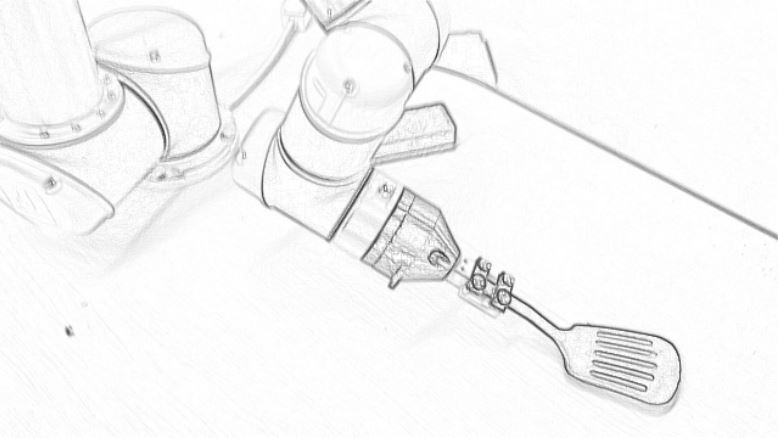
\includegraphics[width=0.60\textwidth]{images/test_image}
\end{figure}
\vspace{0.5 in}
{\centering \huge \color{accentcolor} \sc \textbf{\teamname \\ \productname} \par}
\vspace{0.5 in}
{\centering \large \sc \textbf{\authors} \par}
\newpage


%\vspace{1 in}
%\centerline{January 13th, 2012}
%\newpage

%%% Revision History
\begin{versionhistory}
  	\vhEntry{0.1}{12.04.2017}{LV, JDM}{First draft}
\end{versionhistory}
\newpage

%%% Table of contents
\setcounter{tocdepth}{2}
\tableofcontents
\newpage

%%% List of figures and tables (optional)
\listoffigures
\listoftables
\newpage

%%% Document sections
\section{Introduction}
The UR5 Master Chef is a product that aims to alleviate the need for manual labor in a cooking environment.  The purpose of this design is to provide an interchangeable tool interface allowing for the use of various tools for use in a fast paced food preparation area. The target application for his prototype is to demonstrate the creation, preparation, and serving of grill cheese sandwiches.
\newpage
\section{System Overview}
The main architecture of the system involves 4 main systems communicating with each other. The control logic system and UR5 system pass information with each other via the network system through an Ethernet TCP/IP connection.  The UR5 then provides a signal to the mount system allowing for the docking and undocking of various utensils.

\begin{figure}[h!]
	\centering
 	\includegraphics[width=0.60\textwidth]{images/ADS_layers}
 \caption{A simple architectural layer diagram}
\end{figure}

\subsection{Network}
%%%Each layer should be described separately in detail. Descriptions should include the features, functions, critical interfaces %%%and interactions of the layer. The description should clearly define the services that the layer provides. Also include any %%%%conventions that your team will use in describing the structure: naming conventions for layers, subsystems, modules, and data %%%flows; interface specifications; how layers and subsystems are defined; etc.
This layer contains the router that will allow a connection to the UR5.

\subsection{Control}
This layer contains the camera, raspberry pi that will be use to communicate with the UR5.

\subsection{Mount}
This layer contains the mount that will fit the tool into the mount by controlling the magnet.

\subsection{UR5}
This layer contains the UR5 robot arm, the polyscope(interface), and the control box.
\newpage
\section{Subsystem Definitions \& Data Flow}
This section breaks down your layer abstraction to another level of detail. Here you grapically represent the logical subsytems that compose each layer and show the interactions/interfaces between those subsystems. A subsystem can be thought of as a programming unit that implements one of the major functions of the layer. It, therefore, has data elements that serve as source/sinks for other subsystems. The logical data elements that flow between subsystems need to be explicitly defined at this point, beginning with a data flow-like diagram based on the block diagram.

\begin{figure}[h!]
	\centering
 	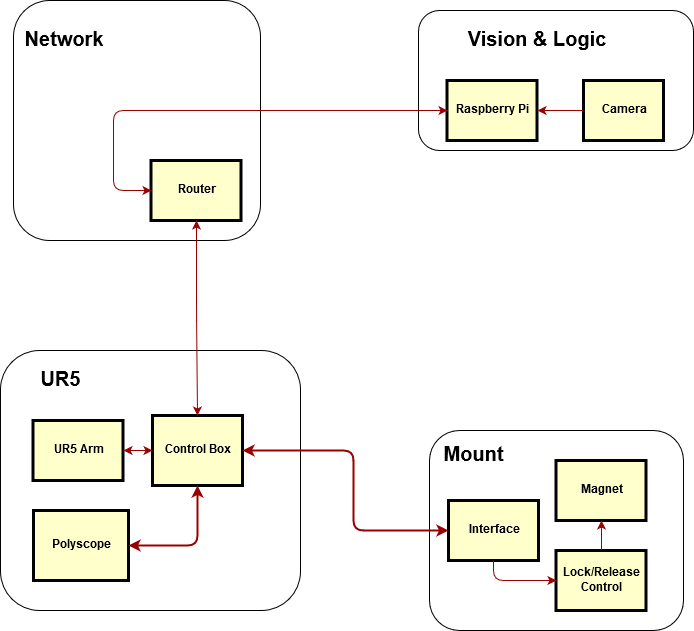
\includegraphics[width=\textwidth]{images/ADS_data_flow}
 \caption{A simple data flow diagram}
\end{figure}

\newpage
\section{X Layer Subsystems}
\input{tex/x_layer_subsystems.tex}
\newpage
\section{Y Layer Subsystems}
\input{tex/y_layer_subsystems.tex}
\newpage
\section{Z Layer Subsystems}
\input{tex/z_layer_subsystems.tex}
\newpage

%%% References
\bibliographystyle{plain}
\bibliographystyle{reference/IEEEtran_custom}
\bibliography{reference/refs}{}

\end{document}